\section{Soddisfacimento degli obiettivi}
Al termine delle 320 ore di \textit{stage} presso \azienda{}, ho potuto effettuare una valutazione complessiva del lavoro svolto, 
focalizzandomi sul grado di raggiungimento degli obiettivi prefissati all'inizio dell'esperienza.

\begin{figure}[!h] 
  \centering 
  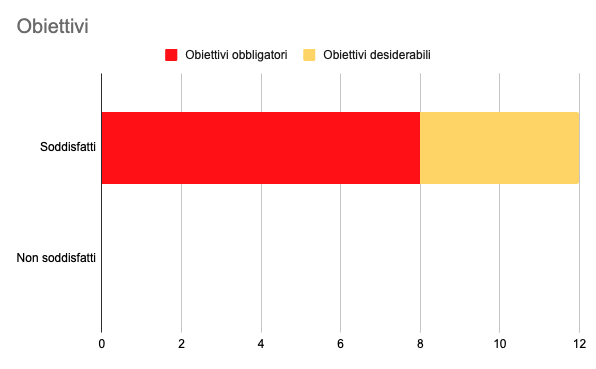
\includegraphics[width=.8\columnwidth]{obiettivi-soddisfatti} 
  \caption{Stato di completamento degli obiettivi.}
  \label{fig:obiettivi-soddisfatti}
\end{figure}

Come mostra la figura \ref{fig:obiettivi-soddisfatti}, sono riuscito a realizzare tutte le funzionalità obbligatorie che il piano di lavoro prevedeva (figura \ref{tab:obiettivi-obbligatori}),
in particolare ho realizzato:
\begin{itemize}
 \item Un \textit{plugin} per Gradle che analizza le dipendenze di un progetto;
 \item Un \textit{database} a grafo per memorizzare le dipendenze;
 \item Un \textit{backend} per esporre le funzionalità del \textit{plugin} tramite API \textit{REST} e per effettuare le interrogazioni al \textit{database};
 \item Un'interfaccia grafica per visualizzare le dipendenze e le relative versioni;
\end{itemize}

Ho realizzato anche tutte le funzionalità desiderabili (\ref{tab:obiettivi-desiderabili}), in particolare:
\begin{itemize}
  \item \textbf{Visualizzazione grafica delle dipendenze:} Sviluppo di una funzionalità che permette di visualizzare 
  le dipendenze di un progetto attraverso una rappresentazione grafica intuitiva. Questo supera il tradizionale formato tabellare, 
  offrendo una comprensione più immediata delle relazioni e delle interdipendenze tra i vari componenti.
  \item \textbf{Integrazione con \textit{repository} remoti per aggiornamenti:} Implementazione di un sistema di integrazione con \textit{repository} remoti, 
  che consente di verificare automaticamente la disponibilità di nuove versioni per le dipendenze utilizzate. 
  Questo assicura che il progetto rimanga aggiornato con le ultime release, migliorando la sicurezza e le prestazioni.
  \item \textbf{Controllo di sicurezza delle dipendenze:} Introduzione di un meccanismo di verifica delle vulnerabilità 
  nelle dipendenze tramite l'integrazione con \textit{repository} remoti. Questo strumento aumenta la sicurezza del \textit{software}, identificando e segnalando eventuali rischi associati alle versioni delle dipendenze in uso.
  \item \textbf{Autenticazione tramite LDAP:} Realizzazione di un sistema di \textit{login} che sfrutta il protocollo LDAP 
  per accedere all'interfaccia grafica. 
   Questo garantisce un livello di sicurezza elevato e una gestione centralizzata delle credenziali utente.
  \end{itemize}

In fine, ho realizzato anche alcune funzionalità aggiuntive, non previste nel piano di lavoro:
\begin{itemize}
  \item \textbf{Esplorazione interattiva dell'albero delle dipendenze:} Implementazione di una funzionalità che consente 
  agli utenti di navigare nell'albero delle dipendenze in modo interattivo e \textit{lazy}. 
  Questo approccio migliora l'esperienza utente, permettendo di caricare e visualizzare le informazioni in maniera 
  efficiente e solo quando necessario.
  \item \textbf{Ricerca di dipendenze con autocomplete:} Sviluppo di un sistema di ricerca avanzato che utilizza 
  l'autocompletamento per suggerire dipendenze in base ai termini inseriti. 
  Questo strumento facilita la ricerca, mostrando un elenco raggruppato di dipendenze corrispondenti,
   migliorando così l'efficienza e la rapidità di selezione.
  \item \textbf{Ricerche avanzate con \textit{query} Cypher:} Creazione di una funzionalità che permette agli utenti di eseguire 
  ricerche di dipendenze utilizzando \textit{query} Cypher. Inserendo la \textit{query} nel campo di ricerca, 
  gli utenti possono ottenere risultati dettagliati in formato JSON. Questo offre un livello di personalizzazione e di 
  dettaglio nella ricerca senza precedenti, adattandosi a esigenze di analisi più complesse.
  \end{itemize}
La pianificazione iniziale delle ore per lo \textit{stage} prevedeva una distribuzione equilibrata tra le diverse fasi del progetto. 
Tuttavia, nel corso dello svolgimento, 
si sono verificate alcune variazioni significative. In particolare, il piano originale allocava circa tre settimane per lo sviluppo 
del \textit{frontend}, basandosi su stime \textit{standard} per questo tipo di lavoro.

Grazie alla mia consolidata esperienza con Angular, sono riuscito a ottimizzare notevolmente i tempi di sviluppo. 
Questa efficienza mi ha permesso di ridurre la durata prevista per questa fase, completando il lavoro in un arco temporale 
inferiore rispetto a quanto pianificato. La conseguenza diretta di questa accelerazione è stata la disponibilità di più 
tempo da dedicare ad altre attività fondamentali.

Ho sfruttato questa opportunità per approfondire la mia conoscenza delle tecnologie emergenti e partecipare a corsi di 
formazione aziendali. Questi corsi, offerti da \azienda{}, hanno arricchito il mio bagaglio di competenze.
